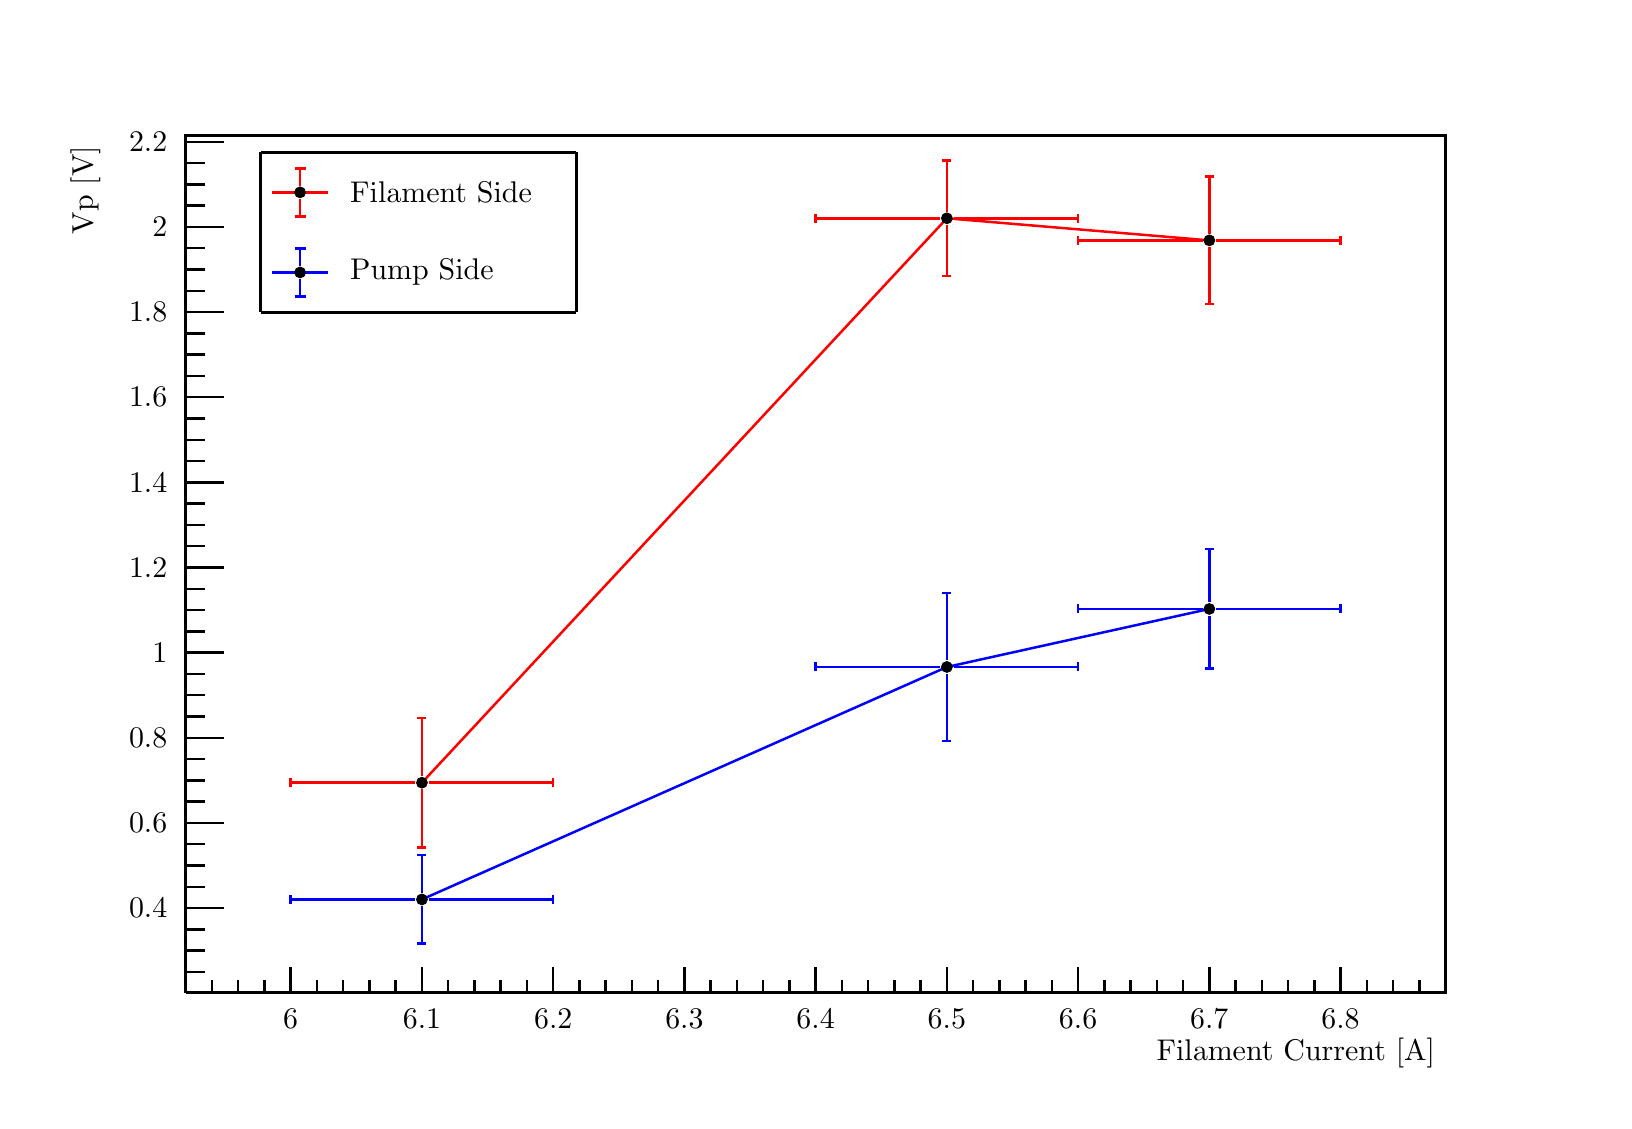
\begin{tikzpicture}
\pgfdeclareplotmark{cross} {
\pgfpathmoveto{\pgfpoint{-0.3\pgfplotmarksize}{\pgfplotmarksize}}
\pgfpathlineto{\pgfpoint{+0.3\pgfplotmarksize}{\pgfplotmarksize}}
\pgfpathlineto{\pgfpoint{+0.3\pgfplotmarksize}{0.3\pgfplotmarksize}}
\pgfpathlineto{\pgfpoint{+1\pgfplotmarksize}{0.3\pgfplotmarksize}}
\pgfpathlineto{\pgfpoint{+1\pgfplotmarksize}{-0.3\pgfplotmarksize}}
\pgfpathlineto{\pgfpoint{+0.3\pgfplotmarksize}{-0.3\pgfplotmarksize}}
\pgfpathlineto{\pgfpoint{+0.3\pgfplotmarksize}{-1.\pgfplotmarksize}}
\pgfpathlineto{\pgfpoint{-0.3\pgfplotmarksize}{-1.\pgfplotmarksize}}
\pgfpathlineto{\pgfpoint{-0.3\pgfplotmarksize}{-0.3\pgfplotmarksize}}
\pgfpathlineto{\pgfpoint{-1.\pgfplotmarksize}{-0.3\pgfplotmarksize}}
\pgfpathlineto{\pgfpoint{-1.\pgfplotmarksize}{0.3\pgfplotmarksize}}
\pgfpathlineto{\pgfpoint{-0.3\pgfplotmarksize}{0.3\pgfplotmarksize}}
\pgfpathclose
\pgfusepathqstroke
}
\pgfdeclareplotmark{cross*} {
\pgfpathmoveto{\pgfpoint{-0.3\pgfplotmarksize}{\pgfplotmarksize}}
\pgfpathlineto{\pgfpoint{+0.3\pgfplotmarksize}{\pgfplotmarksize}}
\pgfpathlineto{\pgfpoint{+0.3\pgfplotmarksize}{0.3\pgfplotmarksize}}
\pgfpathlineto{\pgfpoint{+1\pgfplotmarksize}{0.3\pgfplotmarksize}}
\pgfpathlineto{\pgfpoint{+1\pgfplotmarksize}{-0.3\pgfplotmarksize}}
\pgfpathlineto{\pgfpoint{+0.3\pgfplotmarksize}{-0.3\pgfplotmarksize}}
\pgfpathlineto{\pgfpoint{+0.3\pgfplotmarksize}{-1.\pgfplotmarksize}}
\pgfpathlineto{\pgfpoint{-0.3\pgfplotmarksize}{-1.\pgfplotmarksize}}
\pgfpathlineto{\pgfpoint{-0.3\pgfplotmarksize}{-0.3\pgfplotmarksize}}
\pgfpathlineto{\pgfpoint{-1.\pgfplotmarksize}{-0.3\pgfplotmarksize}}
\pgfpathlineto{\pgfpoint{-1.\pgfplotmarksize}{0.3\pgfplotmarksize}}
\pgfpathlineto{\pgfpoint{-0.3\pgfplotmarksize}{0.3\pgfplotmarksize}}
\pgfpathclose
\pgfusepathqfillstroke
}
\pgfdeclareplotmark{newstar} {
\pgfpathmoveto{\pgfqpoint{0pt}{\pgfplotmarksize}}
\pgfpathlineto{\pgfqpointpolar{44}{0.5\pgfplotmarksize}}
\pgfpathlineto{\pgfqpointpolar{18}{\pgfplotmarksize}}
\pgfpathlineto{\pgfqpointpolar{-20}{0.5\pgfplotmarksize}}
\pgfpathlineto{\pgfqpointpolar{-54}{\pgfplotmarksize}}
\pgfpathlineto{\pgfqpointpolar{-90}{0.5\pgfplotmarksize}}
\pgfpathlineto{\pgfqpointpolar{234}{\pgfplotmarksize}}
\pgfpathlineto{\pgfqpointpolar{198}{0.5\pgfplotmarksize}}
\pgfpathlineto{\pgfqpointpolar{162}{\pgfplotmarksize}}
\pgfpathlineto{\pgfqpointpolar{134}{0.5\pgfplotmarksize}}
\pgfpathclose
\pgfusepathqstroke
}
\pgfdeclareplotmark{newstar*} {
\pgfpathmoveto{\pgfqpoint{0pt}{\pgfplotmarksize}}
\pgfpathlineto{\pgfqpointpolar{44}{0.5\pgfplotmarksize}}
\pgfpathlineto{\pgfqpointpolar{18}{\pgfplotmarksize}}
\pgfpathlineto{\pgfqpointpolar{-20}{0.5\pgfplotmarksize}}
\pgfpathlineto{\pgfqpointpolar{-54}{\pgfplotmarksize}}
\pgfpathlineto{\pgfqpointpolar{-90}{0.5\pgfplotmarksize}}
\pgfpathlineto{\pgfqpointpolar{234}{\pgfplotmarksize}}
\pgfpathlineto{\pgfqpointpolar{198}{0.5\pgfplotmarksize}}
\pgfpathlineto{\pgfqpointpolar{162}{\pgfplotmarksize}}
\pgfpathlineto{\pgfqpointpolar{134}{0.5\pgfplotmarksize}}
\pgfpathclose
\pgfusepathqfillstroke
}
\definecolor{c}{rgb}{1,1,1};
\draw [color=c, fill=c] (0,0) rectangle (20,13.6103);
\draw [color=c, fill=c] (2,1.36103) rectangle (18,12.2493);
\definecolor{c}{rgb}{0,0,0};
\draw [c,line width=0.9] (2,1.36103) -- (2,12.2493) -- (18,12.2493) -- (18,1.36103) -- (2,1.36103);
\definecolor{c}{rgb}{1,1,1};
\draw [color=c, fill=c] (2,1.36103) rectangle (18,12.2493);
\definecolor{c}{rgb}{0,0,0};
\draw [c,line width=0.9] (2,1.36103) -- (2,12.2493) -- (18,12.2493) -- (18,1.36103) -- (2,1.36103);
\draw [c,line width=0.9] (2,1.36103) -- (18,1.36103);
\draw [c,line width=0.9] (3.33333,1.68768) -- (3.33333,1.36103);
\draw [c,line width=0.9] (3.66667,1.52436) -- (3.66667,1.36103);
\draw [c,line width=0.9] (4,1.52436) -- (4,1.36103);
\draw [c,line width=0.9] (4.33333,1.52436) -- (4.33333,1.36103);
\draw [c,line width=0.9] (4.66667,1.52436) -- (4.66667,1.36103);
\draw [c,line width=0.9] (5,1.68768) -- (5,1.36103);
\draw [c,line width=0.9] (5.33333,1.52436) -- (5.33333,1.36103);
\draw [c,line width=0.9] (5.66667,1.52436) -- (5.66667,1.36103);
\draw [c,line width=0.9] (6,1.52436) -- (6,1.36103);
\draw [c,line width=0.9] (6.33333,1.52436) -- (6.33333,1.36103);
\draw [c,line width=0.9] (6.66667,1.68768) -- (6.66667,1.36103);
\draw [c,line width=0.9] (7,1.52436) -- (7,1.36103);
\draw [c,line width=0.9] (7.33333,1.52436) -- (7.33333,1.36103);
\draw [c,line width=0.9] (7.66667,1.52436) -- (7.66667,1.36103);
\draw [c,line width=0.9] (8,1.52436) -- (8,1.36103);
\draw [c,line width=0.9] (8.33333,1.68768) -- (8.33333,1.36103);
\draw [c,line width=0.9] (8.66667,1.52436) -- (8.66667,1.36103);
\draw [c,line width=0.9] (9,1.52436) -- (9,1.36103);
\draw [c,line width=0.9] (9.33333,1.52436) -- (9.33333,1.36103);
\draw [c,line width=0.9] (9.66667,1.52436) -- (9.66667,1.36103);
\draw [c,line width=0.9] (10,1.68768) -- (10,1.36103);
\draw [c,line width=0.9] (10.3333,1.52436) -- (10.3333,1.36103);
\draw [c,line width=0.9] (10.6667,1.52436) -- (10.6667,1.36103);
\draw [c,line width=0.9] (11,1.52436) -- (11,1.36103);
\draw [c,line width=0.9] (11.3333,1.52436) -- (11.3333,1.36103);
\draw [c,line width=0.9] (11.6667,1.68768) -- (11.6667,1.36103);
\draw [c,line width=0.9] (12,1.52436) -- (12,1.36103);
\draw [c,line width=0.9] (12.3333,1.52436) -- (12.3333,1.36103);
\draw [c,line width=0.9] (12.6667,1.52436) -- (12.6667,1.36103);
\draw [c,line width=0.9] (13,1.52436) -- (13,1.36103);
\draw [c,line width=0.9] (13.3333,1.68768) -- (13.3333,1.36103);
\draw [c,line width=0.9] (13.6667,1.52436) -- (13.6667,1.36103);
\draw [c,line width=0.9] (14,1.52436) -- (14,1.36103);
\draw [c,line width=0.9] (14.3333,1.52436) -- (14.3333,1.36103);
\draw [c,line width=0.9] (14.6667,1.52436) -- (14.6667,1.36103);
\draw [c,line width=0.9] (15,1.68768) -- (15,1.36103);
\draw [c,line width=0.9] (15.3333,1.52436) -- (15.3333,1.36103);
\draw [c,line width=0.9] (15.6667,1.52436) -- (15.6667,1.36103);
\draw [c,line width=0.9] (16,1.52436) -- (16,1.36103);
\draw [c,line width=0.9] (16.3333,1.52436) -- (16.3333,1.36103);
\draw [c,line width=0.9] (16.6667,1.68768) -- (16.6667,1.36103);
\draw [c,line width=0.9] (3.33333,1.68768) -- (3.33333,1.36103);
\draw [c,line width=0.9] (3,1.52436) -- (3,1.36103);
\draw [c,line width=0.9] (2.66667,1.52436) -- (2.66667,1.36103);
\draw [c,line width=0.9] (2.33333,1.52436) -- (2.33333,1.36103);
\draw [c,line width=0.9] (2,1.52436) -- (2,1.36103);
\draw [c,line width=0.9] (16.6667,1.68768) -- (16.6667,1.36103);
\draw [c,line width=0.9] (17,1.52436) -- (17,1.36103);
\draw [c,line width=0.9] (17.3333,1.52436) -- (17.3333,1.36103);
\draw [c,line width=0.9] (17.6667,1.52436) -- (17.6667,1.36103);
\draw [anchor=base] (3.33333,0.911891) node[scale=1.08185, color=c, rotate=0]{6};
\draw [anchor=base] (5,0.911891) node[scale=1.08185, color=c, rotate=0]{6.1};
\draw [anchor=base] (6.66667,0.911891) node[scale=1.08185, color=c, rotate=0]{6.2};
\draw [anchor=base] (8.33333,0.911891) node[scale=1.08185, color=c, rotate=0]{6.3};
\draw [anchor=base] (10,0.911891) node[scale=1.08185, color=c, rotate=0]{6.4};
\draw [anchor=base] (11.6667,0.911891) node[scale=1.08185, color=c, rotate=0]{6.5};
\draw [anchor=base] (13.3333,0.911891) node[scale=1.08185, color=c, rotate=0]{6.6};
\draw [anchor=base] (15,0.911891) node[scale=1.08185, color=c, rotate=0]{6.7};
\draw [anchor=base] (16.6667,0.911891) node[scale=1.08185, color=c, rotate=0]{6.8};
\draw [anchor= east] (18,0.598854) node[scale=1.08185, color=c, rotate=0]{Filament Current [A]};
\draw [c,line width=0.9] (2,1.36103) -- (2,12.2493);
\draw [c,line width=0.9] (2.48,2.43665) -- (2,2.43665);
\draw [c,line width=0.9] (2.24,2.70696) -- (2,2.70696);
\draw [c,line width=0.9] (2.24,2.97727) -- (2,2.97727);
\draw [c,line width=0.9] (2.24,3.24759) -- (2,3.24759);
\draw [c,line width=0.9] (2.48,3.5179) -- (2,3.5179);
\draw [c,line width=0.9] (2.24,3.78821) -- (2,3.78821);
\draw [c,line width=0.9] (2.24,4.05852) -- (2,4.05852);
\draw [c,line width=0.9] (2.24,4.32883) -- (2,4.32883);
\draw [c,line width=0.9] (2.48,4.59914) -- (2,4.59914);
\draw [c,line width=0.9] (2.24,4.86945) -- (2,4.86945);
\draw [c,line width=0.9] (2.24,5.13976) -- (2,5.13976);
\draw [c,line width=0.9] (2.24,5.41008) -- (2,5.41008);
\draw [c,line width=0.9] (2.48,5.68039) -- (2,5.68039);
\draw [c,line width=0.9] (2.24,5.9507) -- (2,5.9507);
\draw [c,line width=0.9] (2.24,6.22101) -- (2,6.22101);
\draw [c,line width=0.9] (2.24,6.49132) -- (2,6.49132);
\draw [c,line width=0.9] (2.48,6.76163) -- (2,6.76163);
\draw [c,line width=0.9] (2.24,7.03194) -- (2,7.03194);
\draw [c,line width=0.9] (2.24,7.30226) -- (2,7.30226);
\draw [c,line width=0.9] (2.24,7.57257) -- (2,7.57257);
\draw [c,line width=0.9] (2.48,7.84288) -- (2,7.84288);
\draw [c,line width=0.9] (2.24,8.11319) -- (2,8.11319);
\draw [c,line width=0.9] (2.24,8.3835) -- (2,8.3835);
\draw [c,line width=0.9] (2.24,8.65381) -- (2,8.65381);
\draw [c,line width=0.9] (2.48,8.92412) -- (2,8.92412);
\draw [c,line width=0.9] (2.24,9.19443) -- (2,9.19443);
\draw [c,line width=0.9] (2.24,9.46475) -- (2,9.46475);
\draw [c,line width=0.9] (2.24,9.73506) -- (2,9.73506);
\draw [c,line width=0.9] (2.48,10.0054) -- (2,10.0054);
\draw [c,line width=0.9] (2.24,10.2757) -- (2,10.2757);
\draw [c,line width=0.9] (2.24,10.546) -- (2,10.546);
\draw [c,line width=0.9] (2.24,10.8163) -- (2,10.8163);
\draw [c,line width=0.9] (2.48,11.0866) -- (2,11.0866);
\draw [c,line width=0.9] (2.24,11.3569) -- (2,11.3569);
\draw [c,line width=0.9] (2.24,11.6272) -- (2,11.6272);
\draw [c,line width=0.9] (2.24,11.8975) -- (2,11.8975);
\draw [c,line width=0.9] (2.48,12.1679) -- (2,12.1679);
\draw [c,line width=0.9] (2.48,2.43665) -- (2,2.43665);
\draw [c,line width=0.9] (2.24,2.16634) -- (2,2.16634);
\draw [c,line width=0.9] (2.24,1.89603) -- (2,1.89603);
\draw [c,line width=0.9] (2.24,1.62572) -- (2,1.62572);
\draw [c,line width=0.9] (2.48,12.1679) -- (2,12.1679);
\draw [anchor= east] (1.9,2.43665) node[scale=1.08185, color=c, rotate=0]{0.4};
\draw [anchor= east] (1.9,3.5179) node[scale=1.08185, color=c, rotate=0]{0.6};
\draw [anchor= east] (1.9,4.59914) node[scale=1.08185, color=c, rotate=0]{0.8};
\draw [anchor= east] (1.9,5.68039) node[scale=1.08185, color=c, rotate=0]{1};
\draw [anchor= east] (1.9,6.76163) node[scale=1.08185, color=c, rotate=0]{1.2};
\draw [anchor= east] (1.9,7.84288) node[scale=1.08185, color=c, rotate=0]{1.4};
\draw [anchor= east] (1.9,8.92412) node[scale=1.08185, color=c, rotate=0]{1.6};
\draw [anchor= east] (1.9,10.0054) node[scale=1.08185, color=c, rotate=0]{1.8};
\draw [anchor= east] (1.9,11.0866) node[scale=1.08185, color=c, rotate=0]{2};
\draw [anchor= east] (1.9,12.1679) node[scale=1.08185, color=c, rotate=0]{2.2};
\draw [anchor= east] (0.726934,12.2493) node[scale=1.08185, color=c, rotate=90]{Vp [V]};
\definecolor{c}{rgb}{1,0,0};
\draw [c,line width=0.9] (5,4.02857) -- (11.6667,11.1964) -- (15,10.9159);
\definecolor{c}{rgb}{0,0,0};
\foreach \P in {(5,4.02857), (11.6667,11.1964), (15,10.9159)}{\draw[mark options={color=c,fill=c},mark size=1.921922pt,mark=*] plot coordinates {\P};}
\definecolor{c}{rgb}{1,0,0};
\draw [c,line width=0.9] (4.91404,4.02857) -- (3.33333,4.02857);
\draw [c,line width=0.9] (3.33333,3.97126) -- (3.33333,4.08588);
\draw [c,line width=0.9] (5.08596,4.02857) -- (6.66667,4.02857);
\draw [c,line width=0.9] (6.66667,3.97126) -- (6.66667,4.08588);
\draw [c,line width=0.9] (5,4.11453) -- (5,4.85177);
\draw [c,line width=0.9] (4.94269,4.85177) -- (5.05731,4.85177);
\draw [c,line width=0.9] (5,3.94261) -- (5,3.20537);
\draw [c,line width=0.9] (4.94269,3.20537) -- (5.05731,3.20537);
\draw [c,line width=0.9] (11.5807,11.1964) -- (10,11.1964);
\draw [c,line width=0.9] (10,11.1391) -- (10,11.2537);
\draw [c,line width=0.9] (11.7526,11.1964) -- (13.3333,11.1964);
\draw [c,line width=0.9] (13.3333,11.1391) -- (13.3333,11.2537);
\draw [c,line width=0.9] (11.6667,11.2824) -- (11.6667,11.9324);
\draw [c,line width=0.9] (11.6094,11.9324) -- (11.724,11.9324);
\draw [c,line width=0.9] (11.6667,11.1105) -- (11.6667,10.4604);
\draw [c,line width=0.9] (11.6094,10.4604) -- (11.724,10.4604);
\draw [c,line width=0.9] (14.914,10.9159) -- (13.3333,10.9159);
\draw [c,line width=0.9] (13.3333,10.8586) -- (13.3333,10.9732);
\draw [c,line width=0.9] (15.086,10.9159) -- (16.6667,10.9159);
\draw [c,line width=0.9] (16.6667,10.8586) -- (16.6667,10.9732);
\draw [c,line width=0.9] (15,11.0019) -- (15,11.7246);
\draw [c,line width=0.9] (14.9427,11.7246) -- (15.0573,11.7246);
\draw [c,line width=0.9] (15,10.83) -- (15,10.1073);
\draw [c,line width=0.9] (14.9427,10.1073) -- (15.0573,10.1073);
\definecolor{c}{rgb}{0,0,1};
\draw [c,line width=0.9] (4.91404,2.54584) -- (3.33333,2.54584);
\draw [c,line width=0.9] (3.33333,2.48853) -- (3.33333,2.60315);
\draw [c,line width=0.9] (5.08596,2.54584) -- (6.66667,2.54584);
\draw [c,line width=0.9] (6.66667,2.48853) -- (6.66667,2.60315);
\draw [c,line width=0.9] (5,2.6318) -- (5,3.10725);
\draw [c,line width=0.9] (4.94269,3.10725) -- (5.05731,3.10725);
\draw [c,line width=0.9] (5,2.45988) -- (5,1.98443);
\draw [c,line width=0.9] (4.94269,1.98443) -- (5.05731,1.98443);
\draw [c,line width=0.9] (11.5807,5.49802) -- (10,5.49802);
\draw [c,line width=0.9] (10,5.44072) -- (10,5.55533);
\draw [c,line width=0.9] (11.7526,5.49802) -- (13.3333,5.49802);
\draw [c,line width=0.9] (13.3333,5.44072) -- (13.3333,5.55533);
\draw [c,line width=0.9] (11.6667,5.58398) -- (11.6667,6.43731);
\draw [c,line width=0.9] (11.6094,6.43731) -- (11.724,6.43731);
\draw [c,line width=0.9] (11.6667,5.41206) -- (11.6667,4.55874);
\draw [c,line width=0.9] (11.6094,4.55874) -- (11.724,4.55874);
\draw [c,line width=0.9] (14.914,6.23512) -- (13.3333,6.23512);
\draw [c,line width=0.9] (13.3333,6.17781) -- (13.3333,6.29243);
\draw [c,line width=0.9] (15.086,6.23512) -- (16.6667,6.23512);
\draw [c,line width=0.9] (16.6667,6.17781) -- (16.6667,6.29243);
\draw [c,line width=0.9] (15,6.32108) -- (15,6.99436);
\draw [c,line width=0.9] (14.9427,6.99436) -- (15.0573,6.99436);
\draw [c,line width=0.9] (15,6.14916) -- (15,5.47587);
\draw [c,line width=0.9] (14.9427,5.47587) -- (15.0573,5.47587);
\draw [c,line width=0.9] (5,2.54584) -- (11.6667,5.49802) -- (15,6.23512);
\definecolor{c}{rgb}{0,0,0};
\foreach \P in {(5,2.54584), (11.6667,5.49802), (15,6.23512)}{\draw[mark options={color=c,fill=c},mark size=1.921922pt,mark=*] plot coordinates {\P};}
\definecolor{c}{rgb}{1,1,1};
\draw [color=c, fill=c] (2.95129,10) rectangle (6.96275,12.0344);
\definecolor{c}{rgb}{0,0,0};
\draw [c,line width=0.9] (2.95129,10) -- (6.96275,10);
\draw [c,line width=0.9] (6.96275,10) -- (6.96275,12.0344);
\draw [c,line width=0.9] (6.96275,12.0344) -- (2.95129,12.0344);
\draw [c,line width=0.9] (2.95129,12.0344) -- (2.95129,10);
\draw [anchor= west] (3.95415,11.5258) node[scale=1.08185, color=c, rotate=0]{Filament Side};
\definecolor{c}{rgb}{1,0,0};
\draw [c,line width=0.9] (3.10172,11.5258) -- (3.80373,11.5258);
\draw [c,line width=0.9] (3.45272,11.6117) -- (3.45272,11.8309);
\draw [c,line width=0.9] (3.45272,11.4398) -- (3.45272,11.2206);
\draw [c,line width=0.9] (3.38252,11.8309) -- (3.52292,11.8309);
\draw [c,line width=0.9] (3.38252,11.2206) -- (3.52292,11.2206);
\definecolor{c}{rgb}{0,0,0};
\foreach \P in {(3.45272,11.5258)}{\draw[mark options={color=c,fill=c},mark size=1.921922pt,mark=*] plot coordinates {\P};}
\draw [anchor= west] (3.95415,10.5086) node[scale=1.08185, color=c, rotate=0]{Pump Side};
\definecolor{c}{rgb}{0,0,1};
\draw [c,line width=0.9] (3.10172,10.5086) -- (3.80373,10.5086);
\draw [c,line width=0.9] (3.45272,10.5946) -- (3.45272,10.8138);
\draw [c,line width=0.9] (3.45272,10.4226) -- (3.45272,10.2034);
\draw [c,line width=0.9] (3.38252,10.8138) -- (3.52292,10.8138);
\draw [c,line width=0.9] (3.38252,10.2034) -- (3.52292,10.2034);
\definecolor{c}{rgb}{0,0,0};
\foreach \P in {(3.45272,10.5086)}{\draw[mark options={color=c,fill=c},mark size=1.921922pt,mark=*] plot coordinates {\P};}
\end{tikzpicture}
